% Example report for TTK4250 Group Assignment 2 (factor graph SLAM), written by course staff
% from real runs of the reference solution. Figures: see README.md in this folder.
\documentclass[11pt,a4paper]{article}
\usepackage[margin=2.2cm]{geometry}
\usepackage{fontspec}
\usepackage{amsmath}
\usepackage{graphicx}
\usepackage{booktabs}
\usepackage[font=small,labelfont=bf]{caption}
\usepackage{siunitx}
\usepackage{hyperref}
\usepackage{parskip}

\newcommand{\figref}[1]{Fig.~\ref{#1}}
\newcommand{\tabref}[1]{Table~\ref{#1}}
\newcommand{\book}[1]{(#1) in the book}

\title{TTK4250 Group Assignment 2: Factor graph SLAM\\[2pt]\large Example report}
\author{Group 0: Student A, Student B, Student C}
\date{}

\begin{document}
\maketitle
\vspace{-2em}

\section*{Task 2: Simulated data}

\tabref{tab:sim} lists our sets. Equation numbers refer to the book.

\begin{table}[h]
\centering\footnotesize
\caption{Simulated runs. Noise values are standard deviations per step. NEES and NIS: the average, then the share of per-step values inside the 95\% bounds. The landmark NIS is per degree of freedom (DOF).}
\label{tab:sim}
\setlength{\tabcolsep}{4pt}
\begin{tabular}{lcccccccc}
\toprule
 & \multicolumn{2}{c}{Odometry} & \multicolumn{2}{c}{Measurement} & & & RMSE & \\
\cmidrule(lr){2-3}\cmidrule(lr){4-5}
 & x, y [m] & yaw [°] & range [m] & bearing [°] & \(M/N\) & Mapped / spurious & x, y [m]; yaw [°] & ANEES; ANIS \\
\midrule
S0 & 0.01 & 0.5 & 0.2 & 2.0 & 2/3 & 72 / 3 & 0.72, 0.80; 1.18 & 8.37, 70\%; 0.33, 23\% \\
S1 & 0.05 & 1.0 & 0.05 & 1.0 & 2/3 & 76 / 0 & 0.29, 0.30; 0.48 & 1.91, 99\%; 1.00, 94\% \\
S2 & 0.2 & 4.0 & 0.2 & 4.0 & 2/3 & 76 / 0 & 0.29, 0.30; 0.48 & 0.12, 12\%; 0.06, 0\% \\
S3 & 0.05 & 1.0 & 0.05 & 1.0 & 3/4 & 65 / 7 & 0.83, 0.94; 1.13 & 1.93, 99\%; 1.00, 94\% \\
\bottomrule
\end{tabular}
\end{table}

\paragraph{S0: baseline.} The ANEES is 8.37 against an expected 3, with only 70\% of the NEES inside the bounds, while the landmark NIS sits mostly below its lower bound (\figref{fig:simcons}, left). The pose covariance is too small, so the odometry noise \(Q\) is too small; \(S = HPH^\top + R\) (9.26) is too large, so \(R\) is too large.

\paragraph{S1: better.} We raised \(Q\) and lowered \(R\) until the landmark ANIS reached 1. All errors are more than halved, no landmark is spurious, and both NEES and NIS have about 95\% of their values inside the bounds (\figref{fig:simcons}, right). The MAP estimate minimises (9.6), where each term is weighted by its inverse covariance; the baseline trusts dead reckoning too much and the landmarks too little, so its minimum lies in the wrong place. The ANEES of 1.91 is below its interval [2.85, 3.15], but (4.67) assumes independent terms, and a smoother's pose errors drift slowly over hundreds of steps (\figref{fig:simbirth}). One run averages far fewer independent samples than 999, so we judge consistency by the share inside the bounds.

\paragraph{S2: same errors, inconsistent.} S2 is S1 with every standard deviation multiplied by 4. The estimate is identical to the last digit: multiplying every covariance in (9.6) by 16 divides the cost by 16, which does not move its minimum. Only the covariances change, 16 times too large, so the ANEES drops to 1.91/16 = 0.12 and the ANIS to 0.06. The ratio between \(Q\) and \(R\) decides the estimate; their scale decides whether its covariance, and the association gates built from it, can be trusted.

\paragraph{S3: fewer landmarks.} S3 keeps S1's noise but needs a landmark to be seen in 3 of 4 steps. It maps 11 fewer landmarks, has 7 spurious ones, and its errors are about three times those of S1. Landmarks seen only briefly, at the edge of the field of view, are never confirmed. The yaw error of S3 sits near \(+1°\) for the whole run (\figref{fig:simbirth}). The first landmark is confirmed at step 4 instead of step 1, so the heading drifts on odometry alone for three more steps, and every landmark is initialised from that rotated pose. Only the prior on the first pose ties the map to the world frame, so nothing can undo the rotation later: the map is right relative to itself, but rotated about 1° around the start. At 170\,m that is 3\,m, so far landmarks count as spurious and missed although they agree with their neighbours. The estimate stays consistent: S3's yaw envelope is twice as wide as S1's and covers the offset.

\paragraph{Front-end or back-end?} No set produced a duplicate, so association never failed. S0 and S1 differ in the back-end weighting, S1 and S3 in landmark birth, a front-end decision.

\begin{figure}[p]
\centering
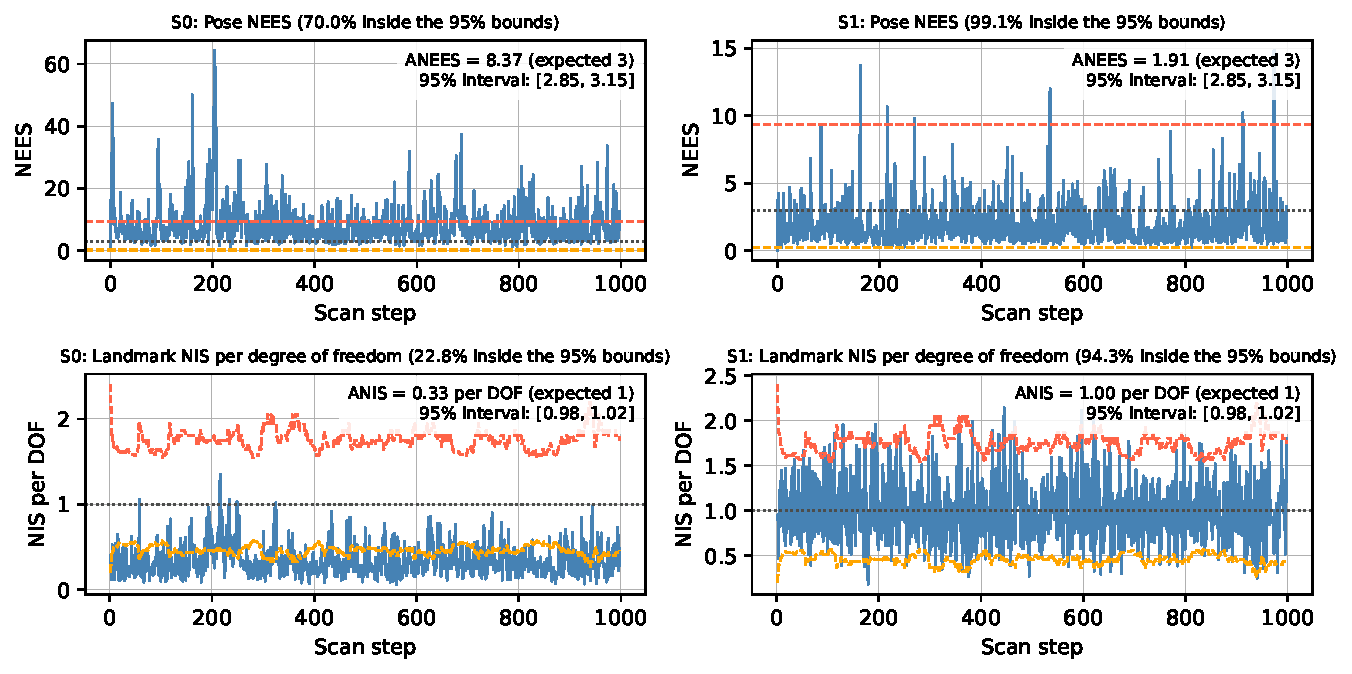
\includegraphics[width=\textwidth]{figures/sim_consistency.pdf}
\caption{Pose NEES (top) and landmark NIS per DOF (bottom) for the baseline S0 (left) and S1 (right). Dashed: 95\% bounds; dotted: expected value.}
\label{fig:simcons}
\vspace{1em}
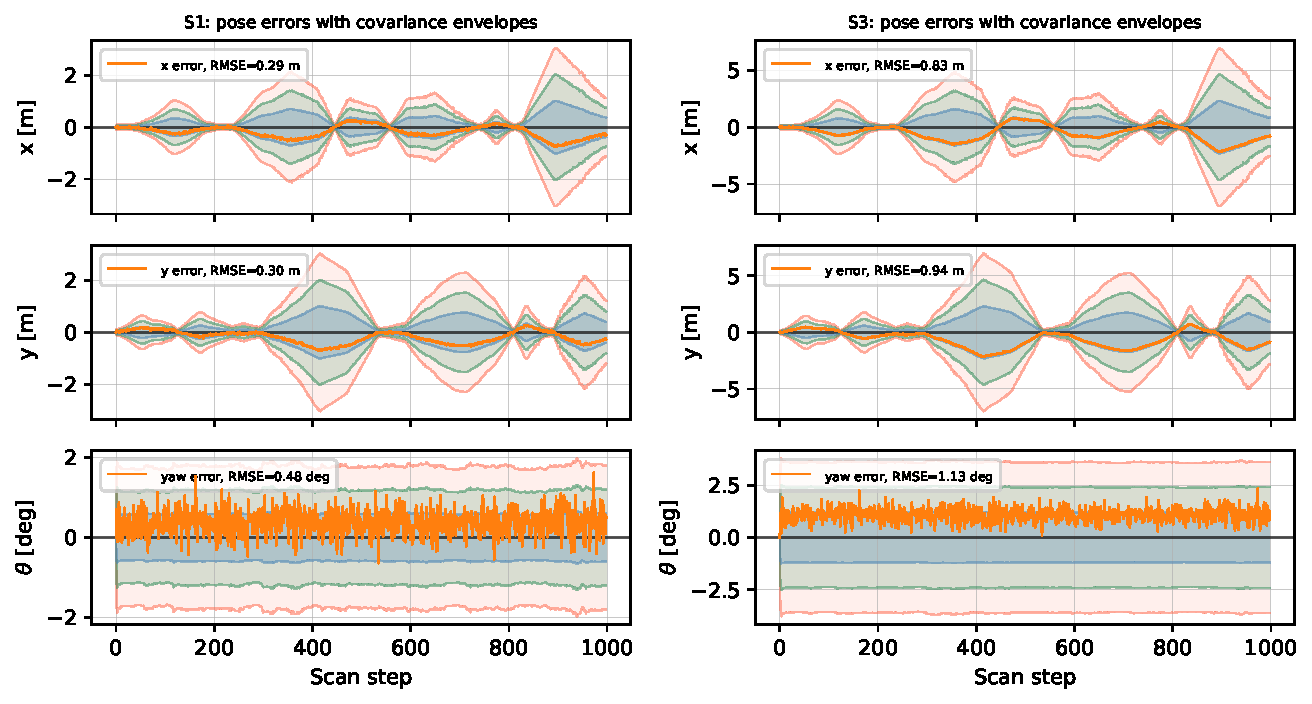
\includegraphics[width=\textwidth]{figures/sim_strict_birth.pdf}
\caption{Pose errors in the body frame for S1 (left) and S3, strict landmark birth (right), with shaded \(1\sigma\), \(2\sigma\) and \(3\sigma\) covariance envelopes. Note the different y-axis scales.}
\label{fig:simbirth}
\end{figure}

\section*{Task 3: Victoria Park}

\begin{table}[h]
\centering\small
\caption{Full Victoria Park runs. The baseline V0 has odometry 0.3\,m, 0.3\,m, 0.6°, range 0.2\,m, bearing 0.5° and both gates at \(\alpha = 0.9999\). ANIS: the average, then the share of per-step values inside the 95\% bounds. GPS distance and GPS NIS only cover times with GPS.}
\label{tab:real}
\begin{tabular}{llcccc}
\toprule
 & Change from V0 & Landmarks & RMS to GPS & GPS ANIS & Landmark ANIS \\
\midrule
V0 & baseline & 288 & 1.79\,m & 2.73, 91\% & 0.26, 24\% \\
V1 & \(R\): 0.1\,m, 0.1°; both \(\alpha = 0.999999\) & 302 & 1.81\,m & 3.07, 88\% & 1.11, 80\% \\
V2 & \(R\): 0.1\,m, 0.1° & 540 & 55.4\,m & 2615, 13\% & 1.04, 79\% \\
V3 & odometry: 0.1\,m, 0.1\,m, 0.3° & 1282 & 218\,m & 42\,326, 3\% & 0.48, 41\% \\
\bottomrule
\end{tabular}
\end{table}

\paragraph{The baseline} works, but most of its landmark NIS values lie below the lower bound (\figref{fig:realcons}): \(R\) is far too large, as in S0.

\paragraph{V2: tight \(R\) breaks.} The landmark ANIS reaches 1.04, yet the map grows to 540 landmarks, pulling away from the baseline within the first 1000 scans (\figref{fig:growth}), and the trajectory ends up 55\,m from the GPS. We believe real tree detections have heavier tails than a Gaussian: trunks are not points, are partly hidden, and their extracted centre shifts with the viewing angle. With a tight \(R\) and a 0.9999 gate, a true re-observation in the tail fails JCBB's test and is born as a new landmark. The duplicate takes constraints the old landmark should have had, loops stop closing, and the drift lets in more duplicates. The NIS cannot show this, as it only covers associated measurements.

\paragraph{V1: the best set.} Raising both gates to 0.999999 lets the tail measurements through: the same \(R\) now gives 302 landmarks, 1.81\,m from the GPS and a landmark ANIS of 1.11 with 80\% inside the bounds instead of 24\%. V1 is as accurate as V0 and close to locally consistent; a wider gate risks wrong associations in clutter, but on this sparse map it costs nothing. The GPS ANIS rises from 2.73 to 3.07 because the tighter \(R\) shrinks the pose covariance. We do not tune for it, as the 1\,m GPS noise is only a guess. The GPS NIS peaks around scans 3800--4200 appear in both runs, so they do not come from the tuning. Neither set gets much closer to the GPS: with 1\,m GPS noise, even a perfect trajectory would be about 1.4\,m away.

\paragraph{V3: low odometry noise.} The run breaks earlier than V2, within 500 scans, and worse: 1282 landmarks and a trajectory 218\,m from the GPS (\figref{fig:realmaps}). With V1's loose gates it still breaks (199\,m, 1191 landmarks), so wider gates do not help; the odometry model is the problem. Wheel odometry errors are not independent from step to step: a wrong wheel radius, a steering offset or slip in a turn bias many consecutive increments the same way. With independent increments the predicted uncertainty grows like \(\sqrt{N}\), but correlated errors grow like \(N\). A large per-step noise covers this; a small one makes the pose overconfident after a long drive, so trees seen again at a loop closure fail the gate and become duplicates. This is the main shortcoming we found: both noise models are white, and on real data neither is. An odometry bias state (e.g.\ a scale factor), or a heavy-tailed measurement model, would allow tight noise without breaking.

\begin{figure}[p]
\centering
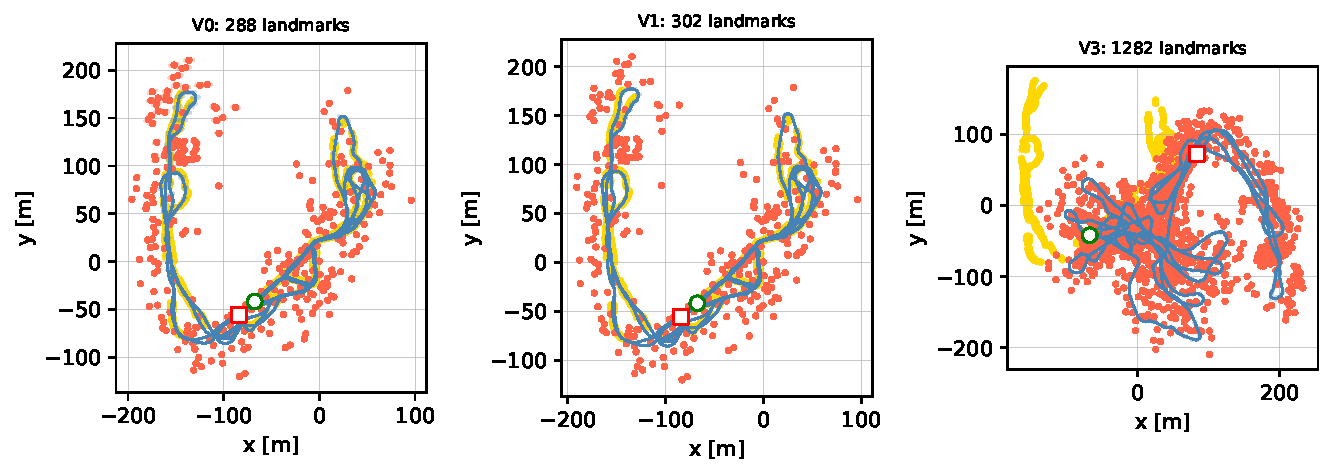
\includegraphics[width=\textwidth]{figures/real_maps.pdf}
\caption{Final trajectory (blue), map (red) and GPS (yellow) for V0, V1 and V3. Note the different axis scales for V3.}
\label{fig:realmaps}
\vspace{1em}
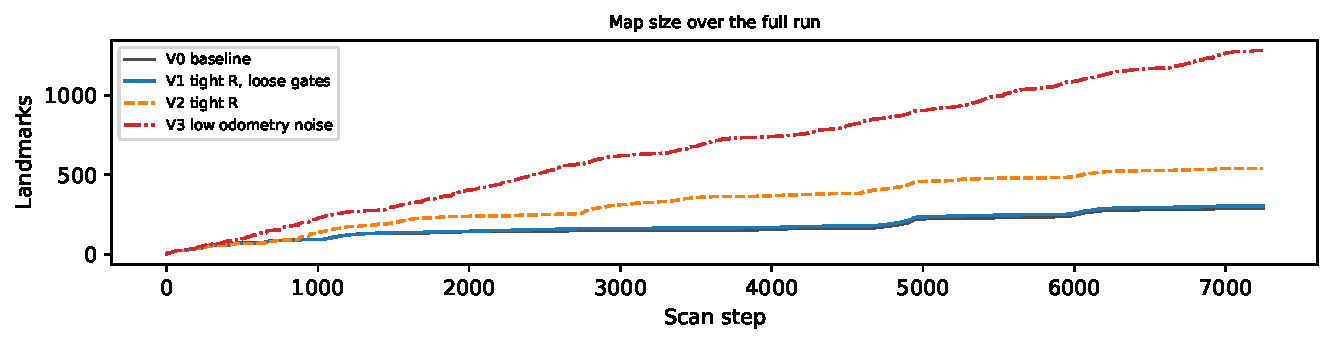
\includegraphics[width=\textwidth]{figures/real_growth.pdf}
\caption{Number of landmarks in the map over the full run.}
\label{fig:growth}
\vspace{1em}
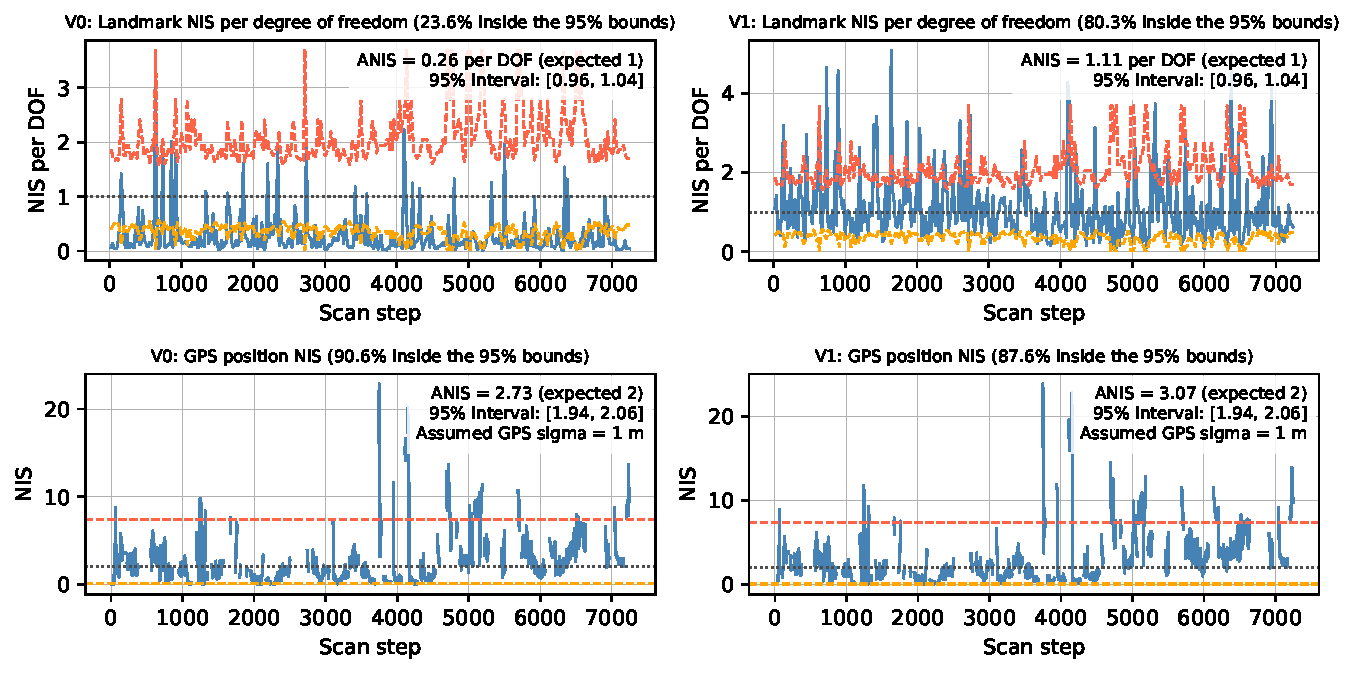
\includegraphics[width=\textwidth]{figures/real_consistency.pdf}
\caption{Landmark NIS per DOF (top) and GPS NIS (bottom) for V0 (left) and V1 (right). Dashed: 95\% bounds; dotted: expected value. The GPS NIS has gaps where the GPS drops out.}
\label{fig:realcons}
\end{figure}

\section*{Task 4: One bad association}

One wrong association at step 600 takes the RMSE from 0.72/0.80\,m to 4.51/5.12\,m and the ANEES from 8.37 to 3794; 61 landmarks are mapped instead of 72, and 73 are spurious instead of 3 (\figref{fig:task4}). At step 600 the NIS per DOF is 1100, as the measurement is compared with a landmark it did not come from. With least squares this one term dominates (9.6), and the optimiser moves the pose and the wrong landmark to explain it. In the next two steps nothing associates, since the true landmarks are no longer where the moved pose predicts them. New landmarks are born from the wrong pose, and from then on the NIS is normal, because they agree with the pose they were initialised from: the NIS checks that the estimate agrees with itself, not with the world. A second map now overlays the first, hence the spurious landmarks. The one sample also lifts the ANIS from 0.33 to 1.33, so the average looks better while the run is far worse.

With Huber, the run matches the baseline: 0.72/0.80\,m, 72 mapped, 3 spurious. The NIS at step 600 is still 1100, as it is computed from the prediction, before the optimisation. What changes is the cost. The wrong measurement is 21\,m off in range and 176° in bearing, a normalised error \(|e|\) of 137. Its least-squares cost \(e^2\) is about 19\,000, and its pull on the estimate, the gradient \(2e\), grows with the error. Huber replaces the cost with \(2\delta|e| - \delta^2\) beyond \(\delta = 1.345\): the gradient is capped at \(2\delta\), which is the same as down-weighting the term by \(\delta/|e| \approx 1\%\). The correct measurements mostly lie inside \(\delta\), so they keep their full weight.

In EKF-SLAM (Sec.~7.2), an update is folded into the mean and covariance and the measurement is discarded. A wrong update cannot be removed afterwards, only covered by inflating the covariance or deleting the affected landmarks, or avoided beforehand by stricter gating or multiple hypotheses. A factor graph keeps every measurement as a factor: a wrong one can be removed later and the graph re-solved, and a robust kernel re-weights every factor at every iteration from its current residual.

\begin{figure}[h]
\centering
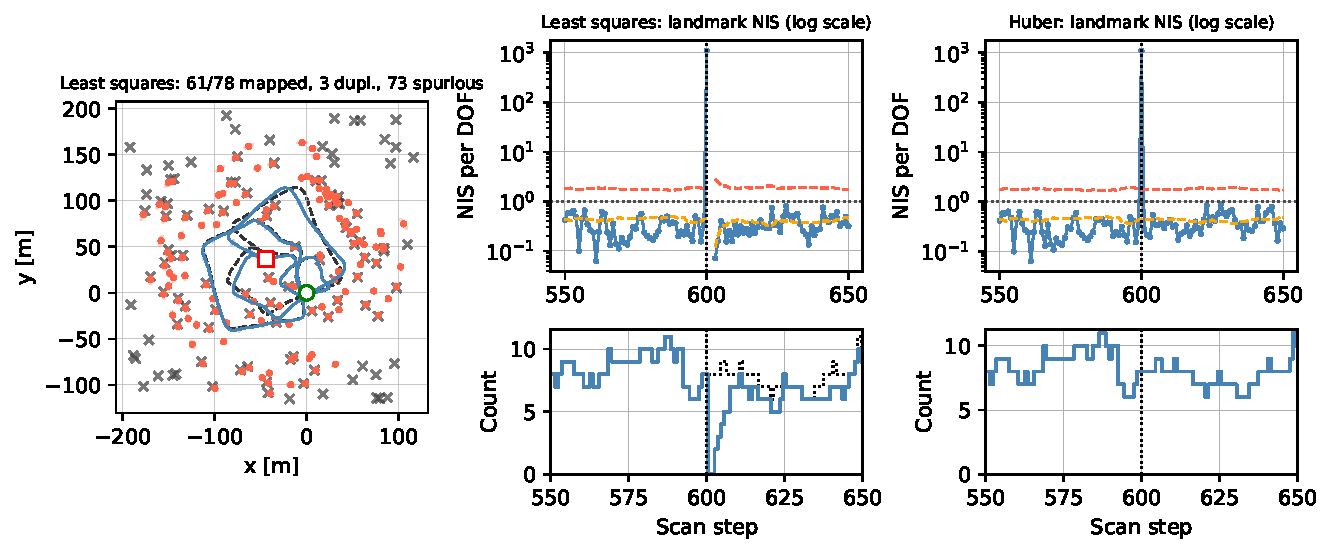
\includegraphics[width=\textwidth]{figures/task4.pdf}
\caption{One wrong association at step 600. Left: final map and trajectory with least squares (dashed: ground truth). Middle and right: \texttt{wrong\_association} for least squares and Huber; top, the landmark NIS per DOF (solid) with its 95\% bounds (dashed) and expected value (dotted); bottom, the number of measurements (dotted) and of associated measurements (solid).}
\label{fig:task4}
\end{figure}

\end{document}
